\subsection{Benchmarks}
\label{sec:Benchmarks}
%\FloatBarrier

In this section, matrix multiply, Sobel edge detection and an image blur
algorithm are used as benchmarks in comparing sequential C++ code, ArBB, EmbArBB, 
and a Haskell library called Repa. 
Repa provides regular shape polymorphic arrays; it permits
parallel execution of the resulting code, making use of multiple
cores, but not of SIMD parallelism~\cite{REPA}.
The Repa versions of the benchmarks used in the comparison 
come from the {\tt repa-examples-3.2.1.1} package on Hackage. 

The processor used for all measurements is a four core Intel Core-I7 930 at 
2.80Ghz. 

\subsubsection{matrix-matrix multiplication}
The matrix multiplication benchmarks consist of square matrices 
of sizes 256x256, 384x384, 512x512, 640x640 and 768x768. 
Figure~\ref{fig:mmchart1} shows the runtimes for the four implementations 
being compared, using the best settings in numbers of cores or threads found 
by previous experiments. The sequential C++ and ArBB versions come 
directly from the ArBB distribution.

\begin{figure}
\includegraphics[width=\linewidth]{./embarbb/img/mmchart1}
\caption{Shows in a log-scale the execution time of matrix-matrix multiplication
         comparing ArBB, EmbArBB, Repa and sequential C++. The ArBB and 
         EmbArBB lines are indistinguishable.}
\label{fig:mmchart1}
\end{figure}

\subsubsection{Sobel edge detection}
In the Repa Sobel code, only the applications of the stencils are timed. This 
part is defined as follows 
\begin{verbatim}
gradientX :: Monad m => Image -> m Image
gradientX img
        = computeP
        $ forStencil2 (BoundConst 0) img
              [stencil2| -1  0  1
                         -2  0  2
                         -1  0  1 |]

gradientY :: Monad m => Image -> m Image
gradientY img
        = computeP
        $ forStencil2 (BoundConst 0) img
             [stencil2|  1  2  1
                         0  0  0
                        -1 -2 -1 |] 
\end{verbatim}

A corresponding EmbArBB code to use in this comparison was implemented.


%\begin{verbatim} 
%gx :: Exp Float -> Exp Float  
%gx x = foldl (+) 0 
%     $ P.zipWith (*) [getNeighbor2D x a b
%                     | (a,b) <- s1] coeffs 

%gy :: Exp Float -> Exp Float 
%gy x = foldl (+) 0 
%     $ P.zipWith (*) [getNeighbor2D x a b
%                     | (a,b) <- s2] coeffs 
%\end{verbatim}

\begin{verbatim} 
gx :: Exp (DVector Dim2 Float) 
    -> Exp (DVector Dim2 Float)  
gx = mapStencil 
         (Stencil [-1,0,1
                  ,-2,0,2
                  ,-1,0,1] (Z:.3:.3)) 

gy :: Exp (DVector Dim2 Float) 
    -> Exp (DVector Dim2 Float) 
gy = mapStencil 
         (Stencil [ 1, 2, 1
                  , 0, 0, 0
                  ,-1,-2,-1] (Z:.3:.3))
\end{verbatim}

%% ** This para needs to be fixed.

We compare these two examples, in which only the applications of the stencils
are timed; we also time the complete Sobel implementation in EmbArBB (shown
in section~\ref{sec:Sobel}).
The Sobel benchmark is run om images of sizes 256x256, 512x512, 1024x1024, 2048x2048 and 4096x4096.
Again, Figure~\ref{fig:sobelchart1} shows that EmbArBB performs well.  As we had expected, the 
Haskell embedding, once a function is captured, seems to impose little or no overhead 
compared to the C++ implementation.

\begin{figure}
\includegraphics[width=\linewidth]{./embarbb/img/sobelchart1}
\caption{Shows in a log-scale the execution time of a key part of the sobel edge 
         detection program. The chart compares EmbArBB to REPA and also displays 
         for reference the execution times of the full sobel program as implemented 
         in section~\ref{sec:Sobel}, called {\em EmbArBB*} in the chart.}
\label{fig:sobelchart1}
\end{figure}

\subsubsection{Blur}

The {\tt blur} benchmark is performed using an algorithm similar to the example 
code in section~\ref{sec:Blur} but with the following changes. The image used
is in RGB color. This means that the stencil needs to be applied three times, 
once to each color plane. Also the image is converted into a form 
where each color intensity is represented by a {\tt Double}. 

Here as well as in the sobel case the Repa code from \newline{\tt repa-examples-3.2.1.1}
times only the actual computational kernel (the application of the stencils) 
including conversion to Doubles. The corresponding EmbArBB part was broken 
out and timed separately as well. The chart~\ref{fig:blurchart} shows comparison
of runtime for the key part of the computation but also adds the full execution 
time of the EmbArBB version (called {\em EmbArBB*} in the chart). 
The full EmbArBB implementation of the blur filter including conversion into Doubles, 
image decomposition into R,G and B planes,  application of the stencil and
reconstructing a planar RGB image in the end.

\begin{figure}
\includegraphics[width=\linewidth]{./embarbb/img/blurchart}
\caption{Shows the execution time of a 7x7 blur filter applied to images 
         of various sizes.}
\label{fig:blurchart}
\end{figure}


%\begin{figure}

\begin{table}
    \begin{small}
    \begin{tabular}{|l|r|r|r|r|}
        \hline
        ~             & 256x256 & 512x512 & 1024x1024 & 2048x2048 \\ \hline
        Repa 3x3      & 12 & 27 &  72 & 190 \\ 
        EmbArBB 3x3   &  1 &  2 &  20 &  77 \\
        EmbArBB* 3x3  &  2 &  9 &  33 & 153 \\  \hline 
        Repa 5x5      & 13 & 32 &  87 & 254 \\
        EmbArBB 5x5   &  1 &  5 &  28 & 105 \\ 
        EmbArBB* 5x5  &  3 & 12 &  46 & 204 \\  \hline 
        Repa 7x7      & 20 & 48 & 119 & 368 \\ 
        EmbArBB 7x7   &  2 & 10 &  46 & 176 \\ 
        EmbArBB* 7x7  &  4 & 17 &  63 & 270 \\
        \hline
    \end{tabular}
    \end{small}
\caption{The table shows execution times (rounded to ms) for various image and stencil size 
         combinations in both Repa and EmbArBB.}
\label{fig:blurtable}

\end{table}


\subsubsection{About the numbers} 
This section presents three benchmarks, two of which compare to Repa only and 
one that compares to Repa, ArBB in C++ and sequential C++ code. In all of these comparisons,
JIT compilation time is excluded.

The comparison to ArBB in C++ shows that the Haskell embedding does not impose any 
extra overhead (at least not in this benchmark); this matched our expectations. More comparisons to the C++ version of ArBB are needed to confirm these first impressions about overhead in the Haskell embedding. If future directions of EmbArBB development develop techniques (such as size inference) that impose a runtime overhead, then the 
comparison in execution to the C++ version becomes more important. 

% ;) 
The comparisons to Repa all show that the performance of EmbArBB compares favourably. This can be attributed to the way in which ArBB's developers at Intel have incorporated vectorisation and threading. 
 

%\end{figure}

%In the Sobel case, EmbArBB and Repa are compared but the complete version 
%of sobel as implemented in section~\ref{sec:Sobel} is also shown for reference. The EmbArBB 
%version of the code is shown earlier in section~\ref{sec:Programming}.






 

%Figures~\ref{fig:arbbchart} and~\ref{fig:embchart} show running times on ArBB and 
%EmbArBB when utilising one,two or four cores. The nearly identical figures 
%illustrate the parallel speedup obtained by ArBB on this particular problem. 

%Figure~\ref{fig:repachart} shows similar parallel speedups for Repa when changing 
%the numbers of threads that it is allowed to use. 

%% ** Maybe need some structuring here.

 

%\begin{verbatim}
%mmultP  :: Monad m
%        => Array U DIM2 Double 
%        -> Array U DIM2 Double 
%        -> m (Array U DIM2 Double)
%
%mmultP arr brr 
% = do   trr      <- transpose2P brr
%        let (Z :. h1  :. _)  = extent arr
%        let (Z :. _   :. w2) = extent brr
%        computeP 
%         $ fromFunction (Z :. h1 :. w2)
%         $ \ix   -> R.sumAllS 
%                  $ R.zipWith (*)
%                        (unsafeSlice arr (Any :. (row ix) :. All))
%                        (unsafeSlice trr (Any :. (col ix) :. All))
%
%transpose2P
%        :: Monad m
%        => Array U DIM2 Double 
%        -> m (Array U DIM2 Double)
%
%transpose2P arr
% = computeUnboxedP
% $ unsafeBackpermute new_extent swap arr
% where  swap (Z :. i :. j)      = Z :. j :. i
%        new_extent              = swap (extent arr)
%
%
%-- | Take the row number of a rank-2 index.
%row :: DIM2 -> Int
%row (Z :. r :. _) = r
%
%
%-- | Take the column number of a rank-2 index.
%col :: DIM2 -> Int
%col (Z :. _ :. c) = c
%
%\end{verbatim}


%\begin{figure}
%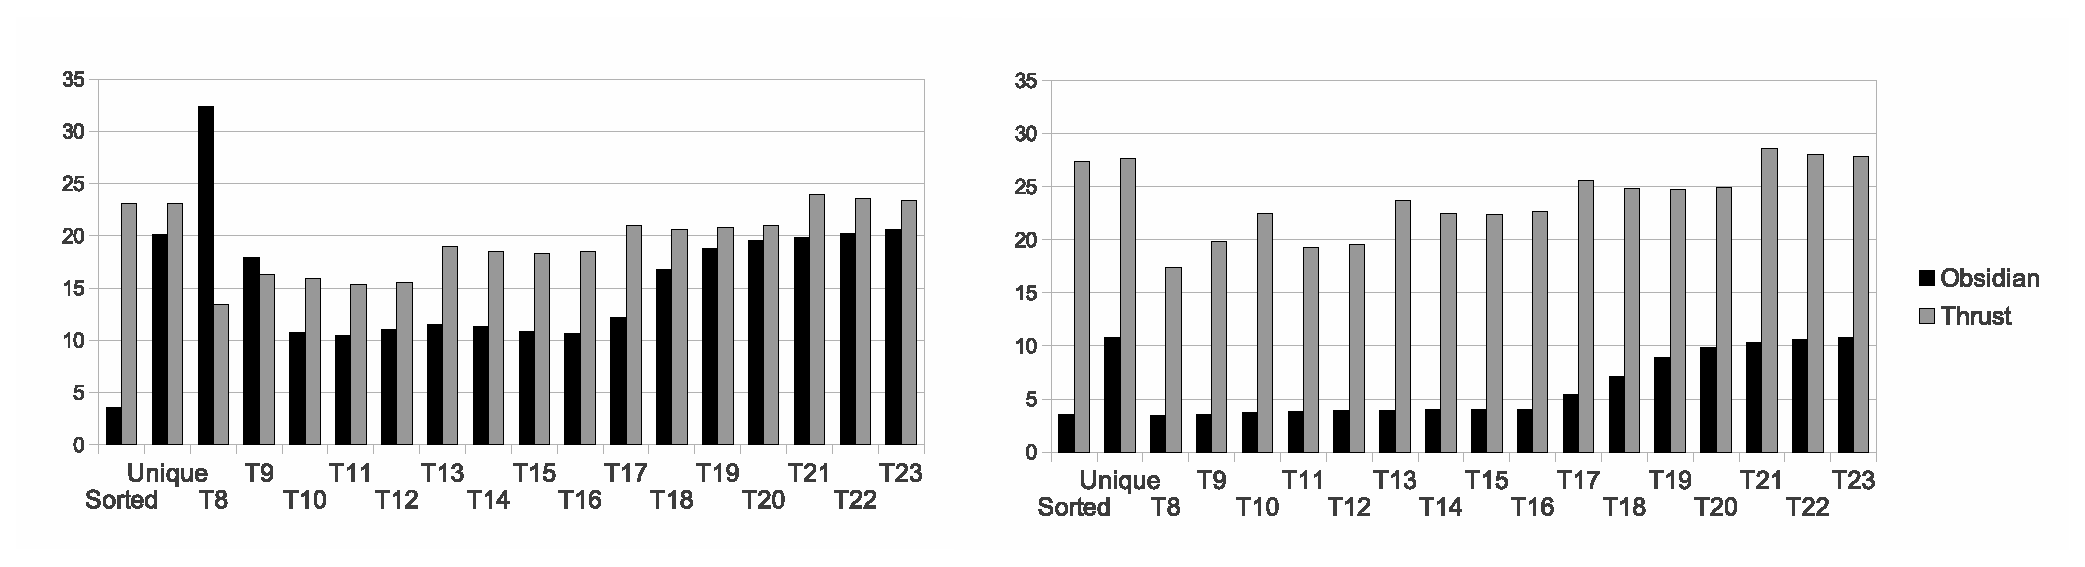
\includegraphics[width=\linewidth]{./img/chart1}
%\caption{Running time and parallel speedup of matrix 
%         multiplication on matrices of different size using ArBB}
%\label{fig:arbbchart}
%\end{figure}


%\begin{figure}
%\includegraphics[width=\linewidth]{./img/arbb1}
%\caption{Execution time for matrix-matrix multiplication using ArBB (C++).
%         Chart shows execution time for various sizes of matrices using 
%         either one two or four cores.}
%\label{fig:arbbchart}
%\end{figure}


%\begin{figure}
%\includegraphics[width=\linewidth]{./img/embarbb1}
%\caption{Execution time for matrix-matrix multiplication using EmbArBB.
%         Chart shows execution time for various sizes of matrices using 
%         either one, two or four cores.}
%\label{fig:embchart}
%\end{figure}

%\begin{figure}
%\includegraphics[width=\linewidth]{./img/repa1}
%\caption{Execution time for matrix-matrix multiplication using Repa.
%         Chart shows execution time for various sizes of matrices using 
%         either one, two, four or eight threads.}
%\label{fig:repachart}
%\end{figure}






%\begin{figure}
%\includegraphics[width=\linewidth]{./img/compare2}
%\caption{CAPTION HERE}
%\label{fig:compare2chart}
%\end{figure}




\FloatBarrier
